\documentclass{template/openetcs_article}
% Use the option "nocc" if the document is not licensed under Creative Commons
%\documentclass[nocc]{template/openetcs_article}
\usepackage{url}
\usepackage{booktabs}
\usepackage[hidelinks]{hyperref}
\usepackage{multicol}
\graphicspath{{./template/}{.}{./images/}{schema/pdf/}}
\begin{document}
\frontmatter
\project{openETCS}

%Please do not change anything above this line
%============================
% The document metadata is defined below

%assign a report number here
\reportnum{OETCS}

%define your workpackage here
\wp{Work-Package 7: ``Toolchain''}


\author{C\'ecile Braunstein}

\affiliation{Bremen University}

\title{Radio Communication Management \\
{\it SRS SUBSET-026-3.5} \\SysML Model}


% define the coverart
\coverart[width=350pt]{chart}

\reporttype{Model Description}

%\begin{document}
\begin{abstract}
%define an abstract here
This document is a part of the model-evaluation project of WP7, it explores
SysML capabilities to provide a (semi)formal model of the SRS SUBSET-026.
\end{abstract}
\maketitle
\tableofcontents
\listoffiguresandtables
\newpage
% ----------------------------------------------------

\section{Short Introduction to Formalism and Tool}
\label{sec:short-intr-form}
This document describes the modeling  of the radio communication management. The
model has been made from the specification description of the SRS SUBSET-026-3.5
 baseline 3 as recommended by D2.5 Methods and tools benchmarking methodology
 \cite{D2-5}.


The formalism used  is SysML \cite{SysML}. More particularly we had used
block diagram, state charts and requirements diagram. 
SysML is a graphical language that extends UML for a customize version suitable
for system engineering. It may help modeling system within a board range of
system variety that may include hardware, software, data, personnel and
facilities. It supports the specification, analysis design, verification and
validation of complex system. 

Enterprise architect (EA) version 9.3 \cite{EA} has been used to implement the
model. Note that this tool is not open source but others tools  such as Papyrus
\cite{papyrus} provides SysML modeling capabilities and are evaluate by others
partners.
EA is a visual platform for designing and constructing
software systems, for business process modeling, and for more generalized
modeling purposes. it covers all aspects of the development cycle. The main
advantages is the requirement management and tracing, the team work and the
include versionning. The main cons : it is not an open source tool.

We had design a test model, this model aims at generate test cases and test
data. The test generator used here is the tool-suite RT-Tester Model-Based generator
(\textsc{Rtt-Mbt}) \cite{Peleska2011,rttmbtreport2011}. It provides sequences of
input data with timing constraints that are used for the stimulation of the
system under test (SUT), concurrently with generated test oracles. 
% ----------------------------------------------------

\section{Modeling Strategy}
\label{sec:modeling-strategy}
Starting from the specification SUBSET-026-chap3.5, we come up with the list of
requirements. The requirements are exactly the text of the SRS. 
This sub-part of the specification defines the management of the radio
communication, e.g. the protocol to follow in order to initiate, 
maintain  and terminate a radio communication. 
From the requirements list, we modeled the set of behaviors defined by direct translation 
into a state chart diagram. In parallel, we implemented  a requirement diagram that
links the requirement list and  the SRS to the model.

An example  figure \ref{fig:methodo-ex} shows an overview of the translation of the specification into a
SysML model. The rest of the document will give  more details on each
object presented. The basic idea is starting from the textual representation, we
can deduce: 
\begin{itemize}
\item Input events : "receives the system version" \\
\verb+MessageIn = SYS_VERSION+
\item Internal variables and constants : "The communication session shall be considered
as established"  \\
\verb+session == ESTABLISHED+
\item Outputs : "shall send a session established report" \\
\verb+MessageOut = SESSION_ESTABLISHED+.
\end{itemize}

\begin{figure}[htbp]
\centering
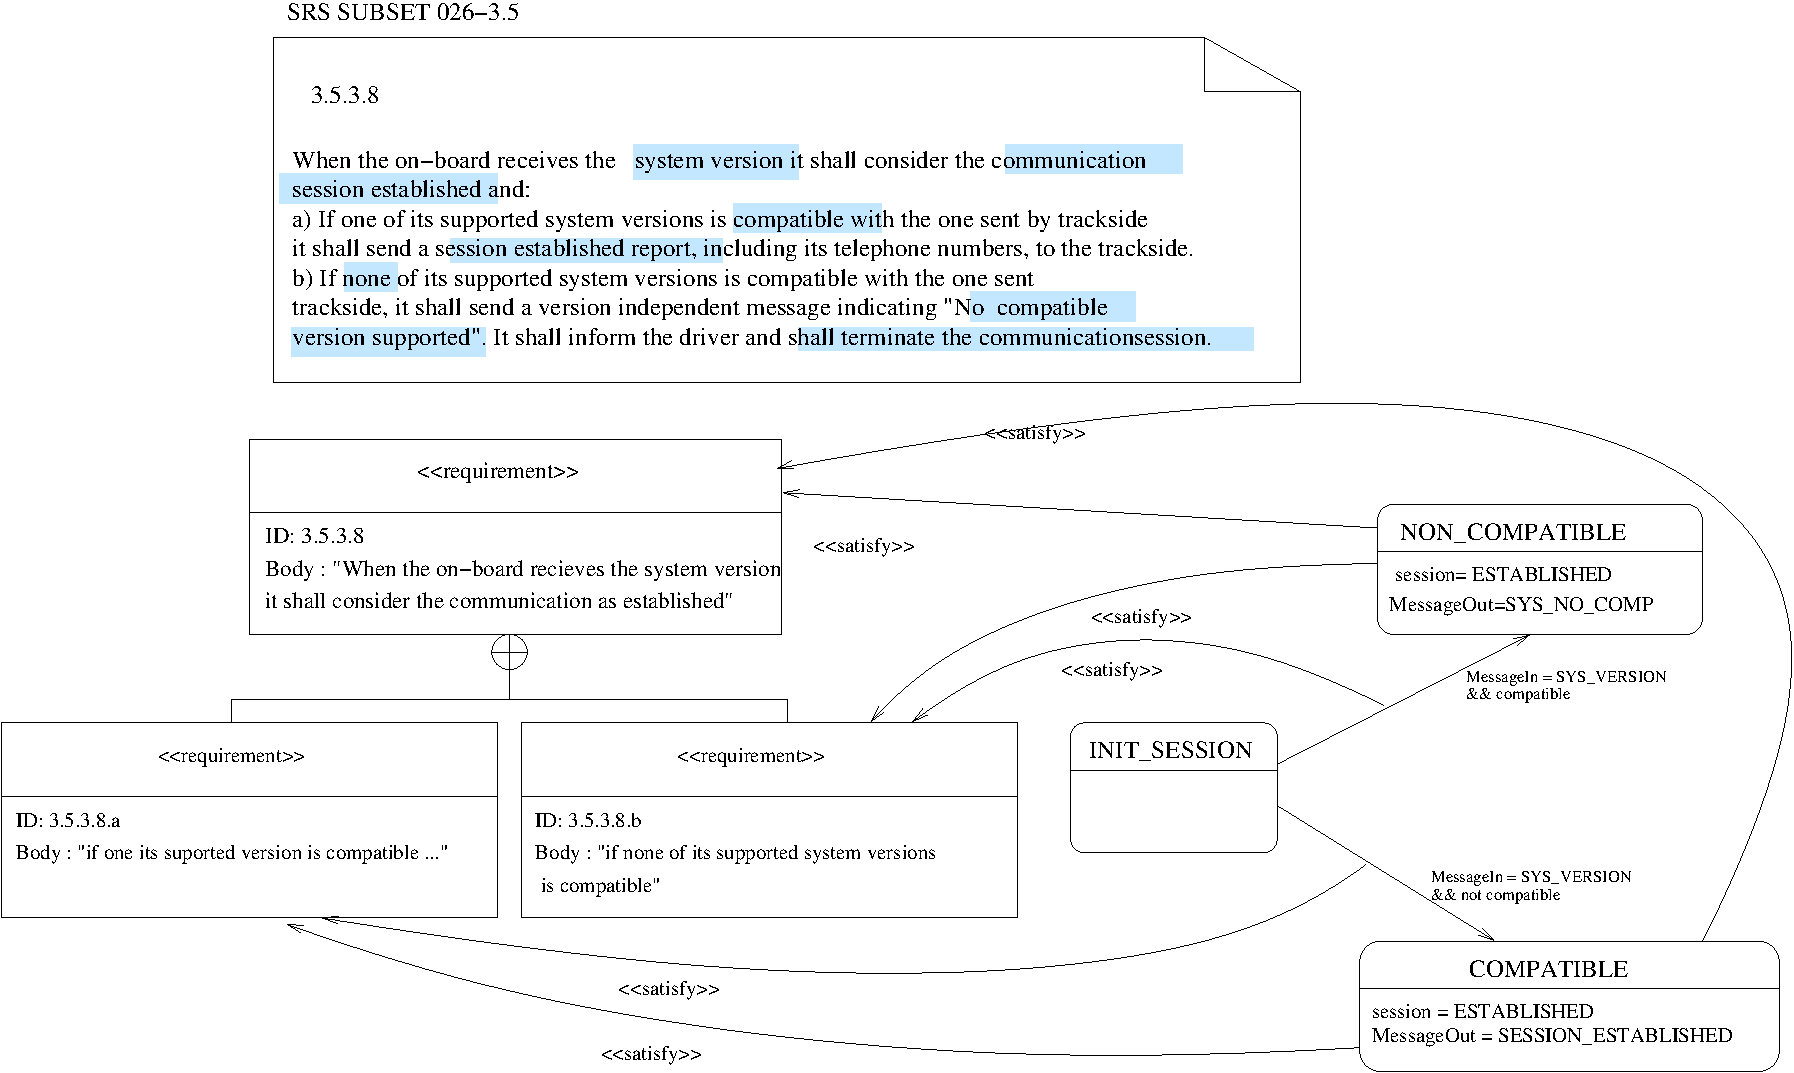
\includegraphics[width=\textwidth]{methodo_example}
\caption{\label{fig:methodo-ex} Methodology example}
\end{figure}

The radio communication management task is part of the set of on-board functions
(see SUBSET-026.4.5). The behavior of this function depends on the result of
others functions such as the function that determine of the ETCS Mode or Level.
This leads us to define an interface between this task
and the other tasks of the on board unit (see section \ref{sec:deta-model-descr}).

Moreover the model is designed for test generation purpose. The model of the
system under test (SUT)  has been
made together with the test execution environment (TE). Here the test
environment is really trivial since it is empty, it allows any possible value
for the inputs of the SUT. One may want to add some constrains on the input
signals or want to sketch some behavior such as an event never happened before
an other one. This may also be model as a state machine.
% ----------------------------------------------------

\section{Model Overview}
\label{sec:model-overview}
The model is composed of two packages : the \emph{system} and the
\emph{requirement}. The system package consists of the SUT model, the TE
model and a set of constants and enumeration types. The
requirement package contains all the requirement and a requirement diagram.

% ----------------------------------------------------

  \subsection{Block and state chart view}
  
The MoRC is the part of the EVC (European vital computer) responsible for the
management of radio communication.
According to the specification this module interacts directly with the following
on-board modules, as shown in figure \ref{fig:arch}: 
\begin{itemize}
\item (DMI) driver module interface~: receives/displays information from/to the driver,
\item (RTM) radio transmission module~: receives/gives commands from/to the radio
network,
\item (BTM) balise transmission module~: sends transmission request from a balise group,
\item (JRU) Juridical recorder unit~: records part of the data exchange for
\item (OBU tasks) other on-board functions (SUBSET-026-4.5) used  by the MoRC such as:
\begin{itemize}
\item track conditions management functions  (SUBSET-026-3.12.1)
that determine for instance if the ETCS system of the track is compatible with the
system on-board.
\item Mode determination (SUBSET-026-3.12.4, SUBSET-026-4.6).

\end{itemize}
\end{itemize}

\begin{figure}[htpb]
\centering
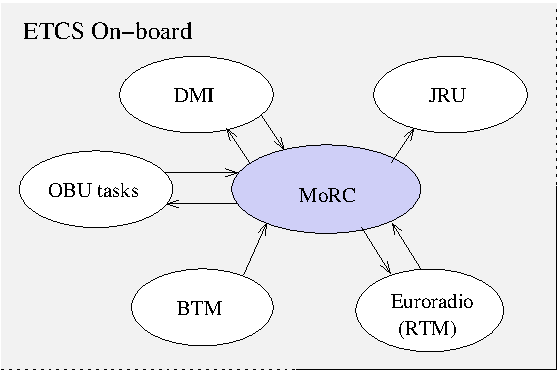
\includegraphics[width =.5\textwidth]{architecture.pdf}
\caption{\label{fig:arch}Interactions between the MoRC and others On-board modules}
\end{figure}

The orders to initiate or terminates a radio communication may come from the
DMI, the BTM, and the RBC (radio block centre) through the RTM. The others OBU
tasks may also order a radio communication (see section \ref{subsec:abstaction}
for more details).

In figure \ref{fig:overview} the MoRC model - \emph{our test model} - is composed
with a the test environment (TE). The inputs and outputs
interfaces are explained in details in section \ref{subsec:inputoutput}.
The test environment abstracts away all the others functions or blocks  which
the SUT may interact with. In our description the test environment is
empty, this means that all possible behavior of the environment may be considered.

\begin{figure}[htpb]
\centering
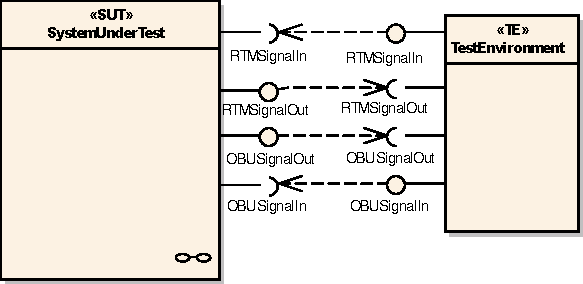
\includegraphics{overview-basicstructure.pdf}
\caption{\label{fig:overview} Model Overview}
\end{figure}

The SUT block consists of two blocks. The SUBSET-026-3.5
specification  separates the management of the radio communication into
3 functions :
\begin{itemize}
\item The session management from chapter 3.5.3 to 3.5.5
\item The registration to the radio network chapter 3.6
\item The safe radio connection indication chapter 3.5.7
\end{itemize}

For the moment we have modeled  the first two items.
The MoRC block and the RadioNetworkRegistration
contains the internal variables used for the protocol implementation and the
state-charts describing their behavior.  The two state machines are
running in parallel.
The two objects interact with each other as shown figure
\ref{fig:sut_interface} and explain later in this document.
\begin{figure}[htpb]
\centering
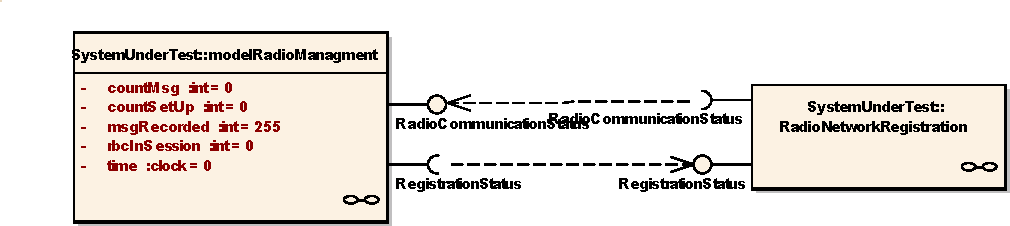
\includegraphics{SystemUnderTest_interface.pdf}
\caption{\label{fig:sut_interface} SUT Overview}
\end{figure}

Until now, the constants used in this chapter and defined in
SUBSET-026.3-A.3.1 are not part of the system under test  block. At this stage of modelisation
it is not defined where they should be declared and recorded to keep track of
possible change or extension. I think they should be part of a special package
regrouping all this kind of information. In the current model they belong to the
system package. 

% ----------------------------------------------------

  \subsection{Requirement view}
  SysML offers a modeling constructs to represent text-based requirements and
relationship with other modeling elements. The requirements in EA diagram may be
described in a graphical or tree structured format. The requirement may also
appear directly other diagram. The diagram requirements  intent to  may be imported and
exported from other tools in csv or XMI format.

In this particular experiment, a table document has been made in csv format from
the SRS.
Each requirement is represented as a number that corresponds to the numbers and bullet points
of the specification document. From this list of requirements, one can directly
find the corresponding paragraph in the documents. We had also added the
complete text in a text attribute  for helping the reader. 



The requirement list is then automatically translate to a requirement package  in SysML where
each requirement is a \emph{requirement} SysML element. Our requirement contains
the following attributes :
\begin{itemize}
\item ID : the corresponding name from the SRS
\item Body: the corresponding text from the SRS
\end{itemize}
Figure \ref{fig:req-example} shows an example of the requirement representation.
\begin{figure}[htbp]
\centering
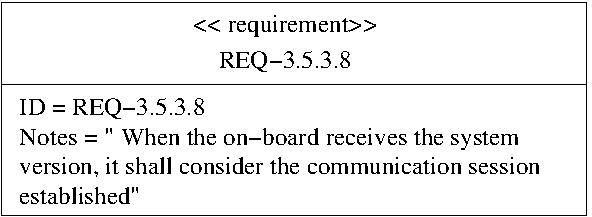
\includegraphics[width=.5\textwidth]{req-example}
\caption{\label{fig:req-example} Example of modeling a requirement}
\end{figure}


Most of requirement refers to the behaviors model as transition of the state-chart
representation.  The link has been made such that each transition satisfy at
least one requirement. Note that in EA, it is not possible to directly link a
transition element to a requirement element, a invariant constraint true has been
added on the transition to make the link.

Others requirement may describe a set of transitions or a more general behavior
property.
In these cases the requirement may be translated as one or more constraints that must be
satisfied by the model. In our model, constraints are invariants expressed in
LTL\cite{PnueliLTL1977}.
SysML does not imposed any language, one can choose other constraints language
such as OCL \cite{ocl2012}.
The following example shows the translation of two requirements into a LTL
properties. The reader should refer to section \ref{sec:deta-model-descr}
for variables and values details.
\begin{description}
\item[REQ-3.5.3.1] "It shall be possible for ERTMS/ETCS on-board equipment and RBC to
initiate a communication session".
\vspace{-1em}
\begin{verbatim}
Finally ((orderOnBoard == 1 || MessageIn == INIT:_SESSION_ORDER || 
MessageIn == INIT_SESSION_TRACK  ) && 
Finally (MessageOut == SESSION_ESTABLISHED))
\end{verbatim}
\end{description}
\begin{description}
\item[REQ-3.5.3.10] "If the establishment of a communication session is
initiated by the RBC, it shall be performed according to the following steps
..."
\vspace{-1em}
\begin{verbatim}
Finally (MessageIn == INIT_SESSION_TRACK && setUp == 1 -> 
Next (MessageOut == SESSION_ESTABLISHED && radioComSession == 1ESTABLISHED)
\end{verbatim}
\end{description}


The requirement diagram only represent the "satisfy" relations between the
requirements and the model. One could refine this diagram and add derive
dependency or containment relationship. Note that in practice we could show the
"satisfy" relations directly on the state-chart view. The separate representation
is more readable. 

% ----------------------------------------------------

\section{Model Benefits}
\label{sec:model-highlights}

In the previous sections, we had describes the use of SysML for modeling
SUBSET-026.3.5. Note that other aspect of the SRS as define in Deliverable D2.5
may also easily represent with SysML. The study here shows the 
modelisation of state charts and timeout. Moreover the arithmetic may be
represented as parametric diagram with constraints block. It is also possible to
use state charts to discretize the behavior of breaking curves.



The benefits of SysML for a semi formal modeling of the SUBSET-026-3.5.
\begin{itemize}
\item General-purpose  modeling languages
\item Can model different domain (arithmetic, state charts ...)
\item Easy export : As an OMG UML 2.0 profile, SysML models are designed to be
exchanged using the XML Meta-data Interchange (XMI) standard.
\item Open source licensee for SysML language
\item Requirements diagram to capture functional and/or performance requirements.
\item Requirements link the SRS to the model
\item Easy data structure definition
\item Customized language via profile, may be use for domain specific purpose
\end{itemize}
Enterprise Architect benefits~:
\begin{itemize}
\item Graphical modeling
\item Different view of the system in one tool
\item List view of all model elements
\item Author, date and status associated to each model element
\item Export/Import facilities
\item Different view for diagrams (Table views,  hierarchy or list view)
\end{itemize}

Some drawbacks~:
\begin{itemize}
\item SysML is only semi-formal
\item EA is not an  open-source software
\item EA needs to work with different tools or plug-in to animate and simulate
the models that are not always using the same XMI definition.
\item The semantic and a glossary should be defined before using SysML
\item EA No requirements table representation
\end{itemize}

% ----------------------------------------------------

\section{Detailed Model Description}
\label{sec:deta-model-descr}
% ----------------------------------------------------
  \subsection{Abstraction}
  \label{subsec:abstaction}
The MoRC model has been made by direct translation of the specification described
in ERTMS subset-026-3.5 In order to keep the complexity low, some
abstractions have been made. The model's behavior would be refined in a next step
of the model's design process. In a first step we focus on the communication
protocol between the MoRC and the RTM. This leads us to abstract some behaviors.

First, our representation will not consider the interfaces with the JRU
since it only recorded existing signals and is not relevant for tests
generation
Secondly, the orders coming from BTM, DMI, EVC will be abstracted as only one message
from the on-board. This message will indicate that a communication session
should be started or be ended. We will not distinguished between the different
events that may occurred since they follow the same connection protocol. Moreover the discrimination
between these events is not well defined in the specification, we will assume
that the decision is taken by another task of the EVC and that the MoRC task only
 starts or terminates a radio communication
Finally, the output messages from MoRC to DMI are not considered for the first version.



% ----------------------------------------------------
  \subsection{Inputs and outputs messages}
  \label{subsec:inputoutput}

Figure \ref{fig:interfaces} shows the messages exchanged at the interface of
the radio communication management module. The numbers in brackets represent the maximal value the message
may have. Note that in a first version the communication will only be set up
with an RBC, communication with a RIU (radio in-fill unit) are not taken
into account.

\begin{figure}[htpb]
\centering
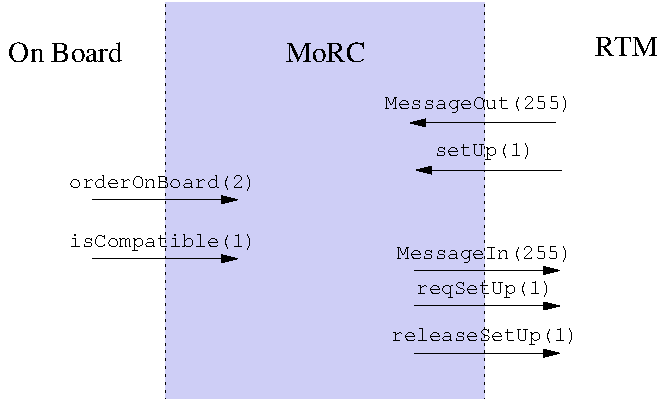
\includegraphics[width =\textwidth]{interface.pdf}
\caption{\label{fig:interfaces} Radio control manager interfaces.}
\end{figure}

\subsubsection{RTM interface}
\verb+MessageToRBC+, \verb+MessageFromRBC+ are the Euroradio messages, their
possible values are defined in the subset-026-8.4 and the subset-026-7.4. The
test cases define by the subset-076 are performed by analyzing the recording of
these messages. In our model we have consider only the relevant messages.
Furthermore, messages are decomposed in variable and packets, these are not
taken into account by our modeling. Our model considers messages only as a number corresponding to an action. 
Table \ref{table:Messages} summarizes the considered messages, the message name
are those used in the model, Id and Packets are those defined in Subset-026-7
and Subset-026-8.

\begin{table}
  \caption{\label{table:Messages} Messages exchange during the Management of
  Radio Communication}
  \begin{tabular}{lclp{.4\textwidth}}\toprule
  Message Name & Id & Packets& Description \\\midrule
  \verb+TERM_SESSION_TRACK+& 24 & Packet 42 ; Q\_RBC = 0& The RBC orders the EVC to {\bf terminate} a communication with RBC \\
   \verb+INIT_SESSION_ORDER+ & 24 &Packet 42 ; Q\_RBC = 1 & 
   The RBC {\bf orders the initiation} of a communication \\
  \verb+SYS_VERSION+ & 32 & & The RBC {\bf acknowledge the initiation} of a
  communication and gives its system version \\
  \verb+INIT_SESSION_TRACK+ & 38 & &  The RBC {\bf initiates} a communication \\
  \verb+TERM_ACK+ & 39 & &  The RBC {\bf acknowledge} the termination
  of a communication \\
  \verb+NETWORK_REG_ORDER+ &  & Packet 45 & The RBC orders the {\bf
    radio network registration}\\    
  \verb+TRANS_OVER_ORDER+ & 131 & & The RBC orders a {\bf transition order} over another RBC \\
  \verb+SYS_NO_COMP+ & 154 &&The EVC {\bf acknowledge the establishment with error}. \\
  \verb+INIT_SESSION+& 155 &&  The EVC {\bf initiates} a communication \\
  \verb+TERM_SESSION+ & 156&&The EVC {\bf terminates} a communication  \\
  \verb+SESSION_ESTABLISHED+ & 159 & & The EVC {\bf acknowledge the establishment} of a communication \\
  \verb+NO_MESSAGE+ & 255 & & No messages are send. \\
  \bottomrule
  \end{tabular}
\end{table}
\begin{description}
\item \verb+NID_RBC_ID+ identifies the RBC it joins the \verb+NID_RBC+ and
\verb+NID_C+ (Subset026-3).
\item \verb+safeRadioCommunication_requestSetUp+,\verb+safeRadioCommunication_setUpEstablished+,\verb+safeRadioCommunication_releaseSetUp+ messages are used for setting
or releasing a safe radio communication.
\item \verb+radioHole_status+ may have the value \verb+MoRC_rhs_begin+, \verb+MoRC_rhs_inside+,
\verb+MoRC_rhs_end+ or
\verb+MoRC_rhs_none+ regarding if the train enters, leaves or is in a announced radioHole 
are compatible.
\item \verb+mobileHWCmd+ represents the
  order to register to a radio network given from the OBU to the radio
  devices.
\item \verb+mobileHWConnectionStatus+  gives the connection status of the mobile
to the radio network.
\item  \verb+actualRadioNetworkID+ is the network ID to register to.
\item \verb+RadioNetworkID_fromTrackside+ is the network ID given by
  the trackside

\end{description}

\subsubsection{Interface with others on board functions}
The different cases to initiate or terminate a communication have been abstract
by a single signal. Since the behavior is the same regardless the different
events, we assume that others tasks of the EVC will activate the signal wen
needed.

\begin{description}
\item \verb+orderFromOnBoard+ represents the order from the on-board EVC to initiate
or terminate a communication. The possible values are the following ones~: 
  \begin{itemize}
  \item \verb+MoRC_obo_noOrder+:  no order;
  \item \verb+MoRC_obo_InitiateCommunication+ represents one of these cases :
	\begin{itemize}
	\item Start of mission procedure,
	\item Report a mode change,
	\item Driver change level to 2 or 3,
	\item End of a radio hole,
	\item The balise group orders a radio communication.
	\end{itemize}
  \item \verb+MoRC_obo_terminateCommunication+ represents one of these cases
	\begin{itemize}
	\item End of mission procedure, 
	\item Driver closes the desk,
	\item Error condition detected on-board.
	\item The balise group orders to end up a radio communication.
	\end{itemize}
 \item \verb+MoRC_obo_registeredNetwork+ orders the radio network registration
  \end{itemize}
\item \verb+systemVersionIsCompatible+ is set to 1 if a the track and the on-board systems
(function system version management)
\item \verb+powerAvailable+ represents if the power is up or down
\item  \verb+memorizeTheLastRadioNetworkID+,
  \verb+RadioNetworkID_fromDriver+ and \verb+RadioNetworkID_memorized+
  are used to register the radio devices to the radio network with
  respects to radio network ID.
\end{description}

The radio management module should take some decision with respect to internal
on-board variables.
This variable are listed blow. The variable definition
are detailed in subset-026-7.
\begin{itemize}
\item \verb+M_LEVEL+ $\in [0..4]$ represents the levels 0,1,2,3 or NTC.
\item \verb+M_ Mode+ $\in[0..16]$ represents the on-board operating mode
computed by mode function (SUBSET-026.4). 
\end{itemize}

% ----------------------------------------------------
\subsection{Internal variables}
\label{subsec:internalvar}


We define a set of variables use for the radio communication management
computation itself.
\begin{itemize}
\item \verb+countSetUp+, \verb+countMsg+, are used to count the number of try
for establishing a radio communication, or to wait for  the acknowledgment
message (SUBSET-026.3.A).
\item \verb+msgRecorded+: Keep track of \verb+MessageFromRBC+
\item \verb+radoComSession+ $\in \{\mathtt{TERMINATED, ESTABLISHED}\}$: indicates if a radio session is established with the track.
\item \verb+time+ used for timeout evaluation
\end{itemize} 
Note that the \verb+safeRadio+ and \verb+radoComSession+ may be used for other
OBU functions like the messages given to the driver or mode computation

The constants or the enumeration type such as Modes name we had  used in the MorC
description are not part of the model itself, they should
belong to a special package.

The communication between the MoRC and the radio network registration
is done by the following interface.
\begin{itemize}
\item \verb+safeRadio+ $\in \{\mathtt{NOCOM, COM, LOST}\}$ indicates if a safe radio communication is on.
\item \verb+mobileSWStatus+ $\in
  \{$\verb+MoRC_mswc_unregistered+,\verb+MoRC_mswc_registering+,\verb+MoRC_mswc_registered+$\}$
  indicates the status of the radio network
\end{itemize}

Note that no
 communication is possible if no network is registered.




% ----------------------------------------------------
  \subsection{Behaviour}
  \label{subsec:behavior}
  The behavior is described figure \ref{fig:behavior}.
A classical transaction starts with an order to established a communication with
an RBC. In this model we assume that the RBC belongs to the RBC accepting list.
Note that we have abstracted the different ways to contact an RBC (last known
number, number entered by the driver ...). Secondly, the MoRC sets up a safe radio
connection, then it initiates a radio communication with the RBC.
An order to terminate a radio communication session may occurred, in this case,
the MoRC sends a termination message to the RBC waits for the acknowledgment and
then releases the safe radio communication.
Our model does not manage the consistency of the successive order, we do not
impose any constraints to when the orders may occur. This may be done by external
tasks.

States \verb+INIT_COM+ and \verb+TERM_COM+ are decomposed as state automaton
handling the maximal number of try and the time out of requests.

Sate \verb+COM+ is decomposed as an automaton, it handles the lost of safe
radio.
\begin{figure}[htpb]
\centering
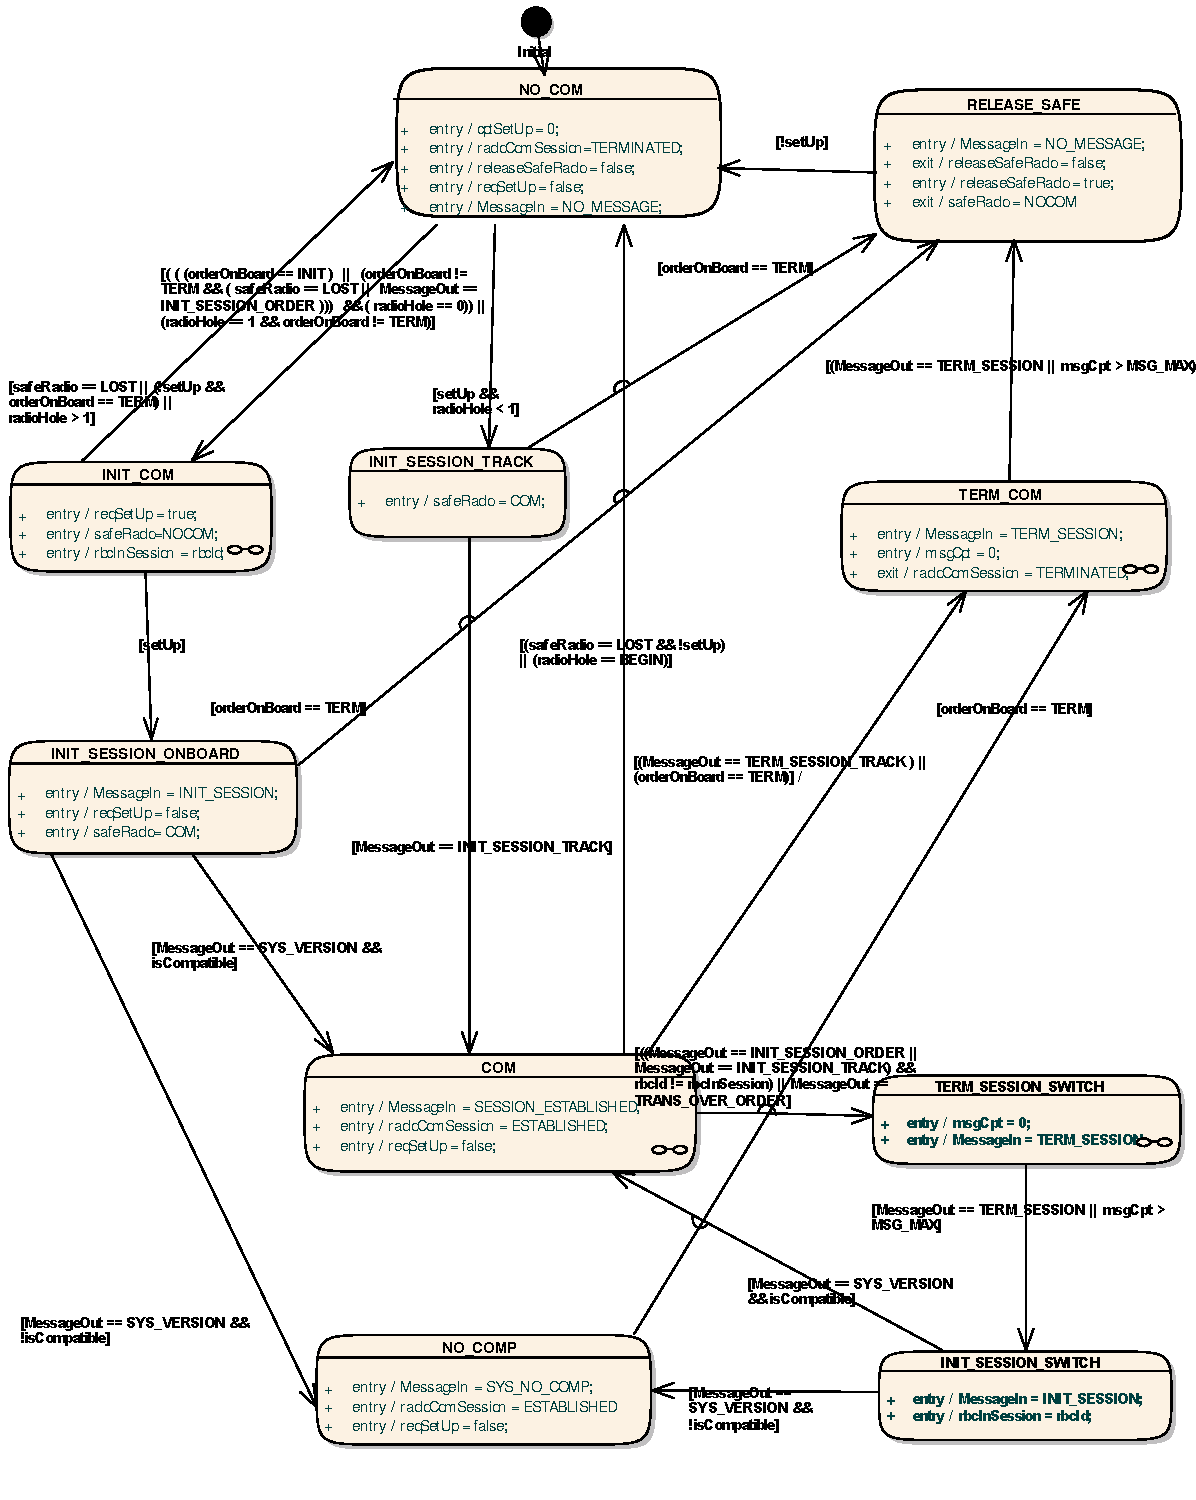
\includegraphics[width=\textwidth]{modelRadioManagment-T.pdf}
\caption{\label{fig:behavior}Automaton of the radio communication management}
\end{figure}



% ----------------------------------------------------
  \subsection{Test cases generation}
  \label{subsec:test_generation}
  \subsection{Tool overview}
\begin{itemize}
\item Purpose
\item Features
\item Certification
\end{itemize}
Paper Certification + bases

The RT-Tester follows the model-based testing approach. 
It provides the following features :
\begin{itemize}
\item Automated Test Case Generation 
\item Automated Test Data Generation 
\item Automated Test Procedure Generation 
\item Automated Requirement Tracing 
\item Test Management system 
\end{itemize}
Starting from a test model design with UML/SYML, the RT-tester fully
automatically generates test cases. They are then specified as test data
(sequences of stimuli with timing constraints) and used to stimulate the SUT and
run concurently with the generated test oracles. The test procedure is the
combination of the test oracles and the SUT composed a test porcdure that can be
compiled and executed.

\FIXME{Basic schema}


\subsection{Test generation}
\begin{itemize}
\item Test coverage
\item Requirement coverage
\item LTL requirement
\end{itemize}



\bibliographystyle{plain}
\bibliography{model}
\end{document}


%%% Local Variables:
%%% mode: latex
%%% TeX-master: t
%%% End:
